\documentclass[a4paper,12pt]{article}
\usepackage{ucs}
\usepackage[utf8x]{inputenc}
\usepackage[russian, english]{babel}  
\usepackage{amsmath}
\usepackage{booktabs}
\usepackage{longtable}
\usepackage[unicode, pdftex]{hyperref}
\usepackage{rotating}
\usepackage{tabularborder}
\usepackage{graphicx}

\graphicspath{ {./figures/} } 

\usepackage[square,numbers]{natbib}
\bibliographystyle{unsrtnat}


\title{Supplement materials}
\author{Mysin I.E.}
\date{}

\begin{document}
\selectlanguage{russian}
\maketitle

\section{Programm instruments}
We have used the simulator Neuron from Python. We have used the code of the models described in the article by Bezaire with coauthors \cite{bezaire_interneuronal_2016} and in Cutsuridis and Poirazi \cite{cutsuridis_computational_2015}. Pyramidal and bistratified neurons were taken from the model of Cutsuridis and Poirazi, the source code of the models was taken from the repository \url{https://github.com/ModelDBRepository/181967}. The remaining neurons are taken from the model of Bezaire, the source code for the neuron models is taken from \url{https://github.com/ModelDBRepository/187604}. The source code of our model is available at \url{https://github.com/ivanmysin/CA1\_rhythms\_model}. \par
%We have used libraries to process the simulated signals: NumPy \cite{2020NumPy-Array}, Scipy \cite{2020SciPy-NMeth}, Elephant \cite{elephant18}. Graphs were plotted with Matplotlib \cite{Hunter:2007}. The code of processing is also available at \url{https://github.com/ivanmysin/CA1\_rhythms\_model}. 

\section{Models of artifitial spike generators}
External inputs to the CA1 field are simulated with artificial spike generators. Almost all neurons in hippocampal formation are modulated by rhythms, therefore we have used von Misses distribution to take phase modulated spike trains:
\begin{equation}
f(\phi) = \frac{exp(\kappa \cdot cos(\phi - \mu) )  }{2\pi \cdot I_0(\kappa) }
\end{equation}
where $I_0(\kappa)$ is the modified Bessel function of order 0. The parameters $\mu$ and $1/\kappa$  are analogous to the mean and variance in the normal distribution. Degree of neuron firing coupling to phase of thythm typicaly is described with parameter $R$ - ray length. Parameter $\kappa$ can be taken from $R$ by following equations \cite{mardia_directional_1999}: 
\begin{equation}
\begin{matrix}
\kappa & = & \left\{
	\begin{matrix}
	2 \cdot R + R^3 + 5/6 \cdot R^5 & \mbox{if } R < 0.53 \\
	-0.4 + 1.39 \cdot R + 0.43 / (1 - R) & \mbox{if } 0.53 \leq   R < 0.85  \\
	1 / (3\cdot R - 4\cdot R^2 + R^3) & \mbox{if } R \geq 0.85 \\
	\end{matrix} \right.
\end{matrix}
\end{equation}
A simple model of spike generator can be presented with an equation:
\begin{equation}
\label{eq:spike_prob_phases}
p_{sp} = \int_\phi^{\phi + \Delta \phi} f(\phi) d \phi
\end{equation}
where $p_{sp}$ is the probabilty of spike generation during $\Delta \phi$. From phases we can go to the time with frequency ($\omega$):
\begin{equation}
\frac{d \phi}{dt} = 2 \pi \omega, \ \phi(t)=2\pi t \omega, \ d\phi=2 \pi \omega dt
\end{equation}
we can join these equations:
\begin{equation}
p_{sp} = S \cdot \int_t^{t + \Delta t} f(2\pi t \omega) 2 \pi \omega dt
\end{equation}
$S$ is a normalization coefficient to get the given spike rate. Each generator is
characterized by the preferred phase ($\mu$), frequency ($\omega$), ray length ($R=0$
is mean that there is no coupling to phase, $R = 1$ is full coupling to phase $\mu$)
and spike rate (regulated by $S$). We add also latency for the generator model, it
is the period after spike generation with zero probability of new spike. We have
used such models for inputs from the medial septum, the lateral entorhinal cortex, and the CA3 field. \par
Neurons of medial entorhinal cortex modulated by theta and gamma
rhythms. We have simulated neurons of the MEC as grid cells. It means
that they show slow periodic activity. It can be simulated as a product of
probabilities simple oscillators:

\begin{equation}
p_{grid} = S \cdot p_{sp}(\omega_{\theta}, \mu_{\theta}, R_{\theta}) \cdot  p_{sp}(\omega_{\gamma}, \mu_{\gamma}, R_{\gamma}) \cdot  p_{sp}(\omega_{grid}, \mu_{grid}, R_{grid})
\end{equation}
All parameters are given below.
Input from the CA3 field is simulated with simple generators and with place cells. The CA3 neurons without place field activity are modulated only by theta rhythm. Place cells are modulated by theta and gamma rhythms, place field is simulated with gaussian:  
\begin{equation}
p_{grid} = S \cdot p_{sp}(\omega_{\theta}, \mu_{\theta}, R_{\theta}) \cdot  p_{sp}(\omega_{\gamma}, \mu_{\gamma}, R_{\gamma}) \cdot 
\frac{exp \Big( \frac{-(t - t_{place})^2}{2 \cdot r_{place}^2}  \Big)}{2 \pi r_{place}}  
\end{equation}
where $t_{place}$ and $r_{place}$ are the center and the radius of a place field in time domain.

\begin{longtable}{llllll}
\caption{Parameters of artifitial generators}\label{ArtifitialCell_parameters}\\
\toprule
{} & ca3\_non\_spatial &  lec & msteevracells & mskomalicells &    msach \\
\midrule
\endhead
\midrule
\multicolumn{6}{r}{{Continued on next page}} \\
\midrule
\endfoot

\bottomrule
\endlastfoot
$R_{\theta}$          &             0.4 &  0.1 &           0.6 &           0.6 &      0.4 \\
$\omega_{\theta}$      &               5 &    5 &             5 &             5 &        5 \\
$latency,\ ms$    &              10 &   10 &             4 &             4 &       10 \\
$\mu_{\theta},\ rad$       &             1.5 &    0 &       $\pi$ &             0 &  $\pi$ \\
$S$ &               5 &    5 &            15 &            15 &        3 \\
\end{longtable}


\begin{longtable}{ll}
\caption{Parameters of artifitial generators}\label{ArtifitialGridCell_parameters}\\
\toprule
{} &    mec \\
\midrule
\endhead
\midrule
\multicolumn{2}{r}{{Continued on next page}} \\
\midrule
\endfoot

\bottomrule
\endlastfoot
$R_{\gamma}$     &    0.4 \\
$R_{grid}$      &    0.9 \\
$R_{\theta}$     &    0.3 \\
$\omega_{grid},\ Hz$ &    0.1 \\
$\omega_{\gamma},\ Hz$ &     63 \\
$\mu_{\gamma},\ rad$    &      0 \\
$latency,\ ms$    &     10 \\
$\omega_{\theta},\ Hz$  &      7 \\
$\mu_{\theta},\ rad$     &  -1.04 \\
$S$ &  1e+08 \\
\end{longtable}


\begin{longtable}{ll}
\caption{Parameters of artifitial generators}\label{ArtifitialPlaceCell_parameters}\\
\toprule
{} & ca3\_spatial \\
\midrule
\endhead
\midrule
\multicolumn{2}{r}{{Continued on next page}} \\
\midrule
\endfoot

\bottomrule
\endlastfoot
$R_{\gamma}$         &         0.6 \\
$R_{\theta}$         &         0.4 \\
$\omega_{\gamma},\ Hz$     &          30 \\
$\mu_{\gamma},\ rad$        &           0 \\
$latency,\ ms$        &          10 \\
$\omega_{\theta},\ Hz$      &           5 \\
$\mu_{\theta},\ rad$         &         1.5 \\
$r_{place}, \ ms$ &        1500 \\
$S$     &       1e+06 \\
\end{longtable}


\section{Neurons models}
\subsection{General notes on neuron models}
All neurons were multi compartments. The potential of each compartment is: 
\begin{eqnarray}
\label{eq:comon_potential}
C\frac{dV}{dt}=-\sum{I_{tm}}-I_{syn} + I_{ext}
\end{eqnarray}
where $C$ is capacity in $\mu F/ cm^2$, $V$ is potential in mV, $t$ is time in ms, $I$ is current in $\mu A/cm^2$. $I_{tm}$ are transmembrane currents, they are described in the following sections, and tables with parameters are given in \ref{tables_of_neurons}. The common equation for transmembrane currents is:
\begin{equation}
I_{tm}= g_{max}\cdot x_1^N\cdot x_2^M \cdot x_3^K \cdot (V-E)
\end{equation}
where $ g_{max}$ is maximal coduntance in $mS/ cm^2$, $E$ is reversal potantial for this channel in $mV$. $x_1,\ x_2, \ x_3$ are the gate variables. All compartments have leak current:
\begin{equation}
I_{L}= g_{L} \cdot (V - E_{L})
\end{equation}
$g_{L}$ and $E_{L}$ are given in tables \ref{tables_of_neurons}.

All gate variables were described with the classical equation: 
\begin{equation}
\frac{dx}{dt} = \frac{x_{\infty}(V) - x}{\tau_x(V)}
\end{equation}
The equations for $x_{\infty}(V)$ and $\tau_x(V)$ are given in the corresponding sections in explicit form or they can be given in form of functions  $\alpha(V)$ and $\beta(V)$
\begin{equation}
\tau_x(V) =  \frac{1}{\alpha(V) + \beta(V)} \ \ \ 
x_{\infty}(V) = \alpha(V) \cdot \tau_x(V)
\end{equation}
Numerical scheme:
\begin{equation}
x_{t + \Delta t} = x_t+\Big(1 - exp \Big(-\frac{\Delta t}{\tau_x} \Big) \Big)\cdot (x_{\infty}-x_t) 
\end{equation}
where $\Delta t = 0.1\ ms$ is integration step.

There is the function \textit{Q(T)} in description of some currents, it is given by:
\begin{equation}
\label{eq:QT}
Q(T)= \frac{F}{ R \cdot T }
\end{equation}
where \textit{R = 8.315\ joule/deg}, \textit{F = 9.648} $\cdot 10^4 \ Coul$,
\textit{T} is the temperature in degrees Kelvin. In all simulations \textit{T=310 deg}.


$I_{syn}$ in equation (\ref{eq:comon_potential}) is a sum of synaptic current, which described in section \ref{synapse_models}. 

External current ($I_{ext}$) in equation (\ref{eq:comon_potential}) simulates noise and influence of very long currents:
\begin{equation}
I_{ext} = I_{ext, mean} + \eta \cdot \sigma_{ext}
\end{equation}
where $I_{ext, mean}$ is a constant value,  $ \eta$ is a random value from normal distribution with mean equals 0 and standard deviation equals 1, $\sigma_{ext}=0.005 \mu A/cm^2/\sqrt{ms}$ is std of noise. To simulate heterogeneously $I_{ext, mean}$ for each neuron is chosen from a lognormal distribution, a mean and std are given below. 

\subsection{CA1 Pyramidal cell}
Pyramid neurons were described using a 15-compartment model (figure \ref{fig:pyr_structures}). The model took into account soma, basal dendrites, and the proximal and distal parts of the apical dendrite. \par
Balance equation for the somatic compartment:
\begin{eqnarray}
C\frac{dV_s}{dt}=-I_L-I_{Na}-I_{kdr}-I_A-I_M-I_H-I_{sAHP}-I_{mAHP}-I_{CaL}- \nonumber \\ -I_{CaT}-I_{CaR}-I_{buff}-I_{syn} + I_{ext}
\end{eqnarray}

Balance equation for the axon:
\begin{equation}
C\frac{dV_a}{dt}=-I_L-I_{Na}-I_{kdr}-I_M-I_{syn}
\end{equation}

Balance equation for the basal dendrites and the proximal part of the apical dendrite:
\begin{eqnarray}
C\frac{dV_{rad,ori}}{dt} =-I_L-I_{Na}-I_{kdr}-I_A-I_M-I_H-I_{sAHP}-I_{mAHP}- \nonumber \\-I_{CaL}-I_{CaT}-I_{CaR}-I_{buff}-I_{syn}+I_{ext}
\end{eqnarray}

Balance equation for the distal part of the apical dendrite:
\begin{equation}
C\frac{dV_{LM}}{dt}=-I_L-I_{Na}-I_{kdr}-I_A-I_{syn}+I_{ext}
\end{equation}
where \textit{I\textsubscript{L}} is the leak current,  \textit{I\textsubscript{Na}} is the fast sodium current, \textit{I\textsubscript{kdr}} is the delayed rectifier potassium current, \textit{I\textsubscript{A}} is the A-type potassium current, \textit{I\textsubscript{M}}
is the M-typepotassium current, \textit{I\textsubscript{H}} is a hyperpolarizing H-type current,
\textit{I\textsubscript{CaL}}, \textit{I\textsubscript{CaT}} and
\textit{I\textsubscript{CaR}} are the L-, T- and R-type \textit{Ca\textsuperscript{2+}} currents, respectively,
\textit{I\textsubscript{sAHP}} and \textit{I\textsubscript{mAHP}} are
slow and medium Ca\textsuperscript{2+} activated K\textsuperscript{+} currents,\textit{ I\textsubscript{buff}}
is a calcium pump/buffering mechanism and \textit{I\textsubscript{syn}} is the synaptic current. \textit{ I\textsubscript{ext}} is the tonic current and noise. The
parameters for all ionic currents are listed in Table \ref{tabel:ca1_pyramidal_cell_parameters}. \par
The sodium current is described by:
\begin{equation}
I_{Na}= g_{max, Na}\cdot m^2\cdot h\cdot s\cdot (V-E_{Na})
\end{equation}
Activation and inactivation kinetics for ${I_{Na}}$ are given by:
\begin{equation}
m_{\infty}=\frac {1}{1+exp(-\frac{V+40} {3})} , \ \ \tau_m=0.05 \ ms
\end{equation}

\begin{equation}
h_{\infty}=\frac {1}{1+exp(\frac{V+45}{3})},  \  \tau_h = 0.5 \ ms,
\end{equation}

\begin{equation}
s_{\infty}=\frac{1+Na_{att}\cdot exp(\frac{V+60}{2})}{1+exp(\frac{V+60}{2})}
\end{equation}


\begin{equation}
\tau_s=\frac{0.00333\cdot  exp(0.0024 \cdot (V+60)\cdot
		Q(T))}{1+exp(0.0012 \cdot (V+60)\cdot Q(T))}
\end{equation}

\textit{Na\textsubscript{att}} variable represents the degree of sodium current
attenuation and varies linearly from soma to distal trunk
\textit{Na\textsubscript{att}} $\in$~[0, 1]: 1 -maximum 0 - zero attenuation (Table \ref{tabel:ca1_pyramidal_cell_parameters}). The delayed rectifier current is given by:

\begin{equation}
I_{Kdr} = g_{Kdr} \cdot m^2 \cdot (V-E_K)
\end{equation}

\begin{equation}
m_{\infty}=\frac{1}{1+exp(-\frac{V+42}{2})}, \tau_m = 2.2 \ ms
\end{equation}

The sodium and delayed rectifier channel properties are slightly different in the soma, axis and dendritic arbor. The $m_{\infty}$ and $h_{\infty}$
somatic/axonic HH channel kinetics as well as the time constants for both $I_{Na}^{sa}$ and $I_{Kdr}^{sa}$, are modified as follows. For the sodium:

\begin{equation}
m_{\infty}^{sa}=\frac {1}{1+exp(-\frac{V+44}{3})} ,\ \ 
h_{\infty}^{sa}=\frac {1}{1+exp(\frac{V+49}{3.5})}
\end{equation}

while for the potassium delayed rectifier

\begin{equation}
m_{\infty}^{sa}=\frac {1}{1+exp(-\frac{V+46.3}{3})}
\end{equation}

The time constant for somatic and axonic \textit{Na\textsuperscript{+}}~channel activation is kept the
same $\tau$\textsubscript{m} = 0.05 ms while for inactivation is set to $\tau$\textsubscript{h}= 1 ms. The $\tau$-value for the delayed rectifier channel activation is set to $\tau_{m}= 3.5 ms$.
The fast inactivating A-type K\textsuperscript{+} current is described by
\begin{equation}
I_A = g_{max, A} \cdot n \cdot l \cdot (V - E_K)
\end{equation}

\begin{equation}
n_{\infty} = \frac{\frac{-0.01(V+21.3)}{exp(-(V+21.3)/35)-1}}{\frac{-0.01(V+21.3)}{exp(-(V+21.3)/35)-1} + \frac{0.01(V+21.3)}{exp( (V+21.3)/35)-1} } \ \ \tau_n=0.2 \ ms
\end{equation}

\begin{equation}
l_{\infty} = \frac{\frac{-0.01(V+58)}{exp( (V+58)/8.2)-1}}{\frac{-0.01(V+58)}{exp( (V+58)/8.2)-1} + \frac{0.01(V+58)}{exp(-(V+58)/8.2)-1}}
\end{equation}

\begin{equation}
\begin{matrix}
\tau_l & =
& \left\{
\begin{matrix}
5+2.6(V+20)/10 & \mbox{if } V > 20 mV \\
5 & \mbox{otherwise }
\end{matrix} \right.
\end{matrix}
\end{equation}


The hyperpolarizing H-current is:
\begin{equation}
I_H=g_{max, H} \cdot H \cdot (V-E_H)
\end{equation}

\begin{equation}
H_{\infty }=\frac {1}{1+exp((V-V_{half})/8)}  
\end{equation}

\begin{equation}
\tau_{H}=\frac{exp( 0.003364\cdot
	(V-V_{halft})}{0.05 \cdot q10^{(T-33)/10} \cdot
	(1+a_{H})}
\end{equation}


\begin{equation}
a_{H}=exp( 0.008316 \cdot (V-V_{halft}))
\end{equation}
where \textit{q10} =  0.4, \textit{V\textsubscript{halft}}
see in Table \ref{tabel:ca1_pyramidal_cell_parameters}.

The slowly activating voltage‑dependent potassium current, \textit{I}\textit{\textsubscript{M}},~is given by the
equations:


\begin{equation}
I_m=10^{-4}\cdot T_{adj}(T)\cdot g_m\cdot m\cdot
(V-E_K)
\end{equation}


\begin{equation}
\alpha_m =  \frac{10^{-3}\cdot(V+30)}{(1-exp(-(V+30)/9))T_{adj}(T)} 
\end{equation}
\begin{equation}
\beta_m = \frac{ -10^{-3}\cdot(V+30)}{(1-exp((V+30)/9))T_{adj}(T)}
\end{equation}
\begin{equation}
T_{adj}(T)=2.3^{(T - 287)/10}
\end{equation}


The slow after-hyperpolarizing current, is given by equations:
\begin{equation}
I_{sAHP}= g_{max, sAHP} \cdot m^3 \cdot (V-E_K)
\end{equation}

\begin{equation}
\frac{dm}{dt}=\frac{\frac{Cac}{(1+Cac)}-m}{\tau_m}
\end{equation}

\begin{equation}
\tau_m=max \Big(\frac {1}{0.003 \cdot (1+Cac)\cdot 3^{(\text{deg}C-22)/10}}, \ 0.5 \Big)
\end{equation}
where 
$Cac=(40 \cdot [Ca^{2+}]_{in})^2$.

The medium after-hyperpolarizing current, I\textsubscript{mAHP} is:

\begin{equation}
I_{mAHP}= g_{max, mAHP}\cdot m\cdot (V-E_K)
\end{equation}

\begin{equation}
\alpha_m(V)=\frac{0.48}{1+\frac{0.18}{[Ca^{2+}]_{in}}\cdot exp(-1.68\cdot V\cdot Q(T))}
\end{equation}

\begin{equation}
\beta_m(V)=\frac{0.28}{1+\frac{[Ca^{2+}]_{in}}{0.011\cdot exp(-2\cdot V\cdot Q(T))}}
\end{equation}

Q(T) see formula (\ref{eq:QT}). \par
The somatic high-voltage activated (HVA) L-type Ca\textsuperscript{2+} current is given by


\begin{equation}
I_{CaL}^s= g_{max, CaL}^s\cdot m\cdot \frac{0.001 \cdot ghk(V, [Ca^{2+}]_{in}, [Ca^{2+}]_{out}) }{0.001 + [Ca^{2+}]_{in}}
\end{equation}

\begin{equation}
\alpha_m(V)= \frac{-0.275 \cdot (V+27.01)}{exp(-(V+27.01)/3.8)-1}
\end{equation}

\begin{equation}
 \beta_m(V)= 4.7 \cdot exp(-(V+63.01)/17)
\end{equation}


whereas the dendritic L-type calcium channels have different kinetics: 


\begin{equation}
I_{CaL}^d= g_{max, CaL}^d \cdot m^3 \cdot h \cdot
(V-E_{Ca})
\end{equation}

\begin{equation}
m_{\infty}(V)=\frac {1}{1+exp(-(V+37))}
\end{equation}
\begin{equation}
h_{\infty}(V)=\frac {1}{1+exp( (V+41)/0.5)}
\end{equation}

Their time constants are equal to $\tau_m$ = 3.6 \textit{ms} and $\tau_h$=29 \textit{ms}. The low-voltage activated (LVA) T-type Ca\textsuperscript{2+} channel kinetics are given by equations:
\begin{equation}
I_{CaT} = g_{max, CaT}\cdot m^2\cdot h \cdot \frac{0.001 \cdot ghk(V,[Ca^{2+}]_{in},[Ca^{2+}]_{out})}{0.001+[Ca^{2+}]_{in} }
\end{equation}

\begin{eqnarray}
ghk(V,\ [Ca^{2+}]_{in},\ [Ca^{2+}]_{out}) = \nonumber \\
= -x\cdot (1 - [Ca^{2+}]_{out}/[Ca^{2+}]_{in} \cdot exp(V/x)) \cdot f(V/x)
\end{eqnarray}

\begin{equation}
x=\frac{0.0853\cdot T}{2}, \\
f(z) = \begin{cases} 1-\frac {z}{2}, & if \ |z|<10^{-4} \\ \frac z{e^z-1}, & \  otherwise \ \end{cases}
\end{equation}

\begin{equation}
\alpha_m(V)=-0.196\cdot \frac{(V-19.88)}{exp(-(V-19.88)/10)-1} 
\end{equation}

\begin{equation}
\beta_m(V) = 0.046\cdot exp(-(V/22.73))
\end{equation}

\begin{equation}
\alpha_h(V)= 0.00011\cdot exp(-(V+57)/19)
\end{equation}
\begin{equation}
\beta_h(V)=\frac {0.68}{exp(-(V-15)/10)+1}
\end{equation}
where $[Ca^{2+}]_{in}$ and $[Ca^{2+}]_{out}$ are the internal and external calcium concentrations. The HVA R-type Ca2+ current is described by:
\begin{equation}
I_{CaR} = g_{max, CaR}\cdot m^3\cdot h\cdot (V-E_{Ca})
\end{equation}

 There is the difference between somatic and dendritic CaR currents in the $\alpha(V)$, $\beta(V)$ and $\tau$ ~parameter values. For the somatic current, $\tau_m$ = 100 \textit{ms} and $\tau_h$ = 5\textit{ms} while for the dendritic current $\tau_m$ = 50 \textit{ms} and $\tau_h$=5 \textit{ ms}. The $\alpha(V)$ and $\beta(V)$ equations for dendritic CaR channels are:

\begin{equation}
m_{\infty}(V)=\frac {1}{1+exp(-(V+48.5)/3)}
\end{equation}
\begin{equation}
h_{\infty}(V)=\frac {1}{1+exp(V+53)}
\end{equation}
while for the CaR channels of the soma:
\begin{equation}
m_{\infty}(V)=\frac {1}{1+exp(-(V+60)/3)}
\end{equation}
\begin{equation}
h_{\infty}(V)=\frac {1}{1+exp(V+62)}
\end{equation}

There is a calcium pump/buffering mechanism in the cell body and along the apical and basal trunk. The factor for $Ca^{2+}$ entry was changed from \textit{f\textsubscript{e}} = 10,000~to \textit{f\textsubscript{e}} = 556 ~and the rate of calcium removal was made 7 times faster. The kinetic equations are given by:

\begin{equation}
Ca_{input flow} = \begin{cases} \frac{-f_e \cdot I_{Ca, sum} }{0.2 \cdot F}, & if \ Ca_{input flow} > 0  \\ 0, & \  otherwise \ \end{cases}
\end{equation}

\begin{equation}
\frac{d[Ca^{2+}]_{in}}{dt}=Ca_{input flow} +\frac{[Ca^{2+}]_{0}-[Ca^{2+}]_{in}}{\tau_{Ca}}
\end{equation}

$[Ca^{2+}]_{0} = 10^{-4} \ mM, \ \tau_{Ca} = 1400 \ ms$


\bigskip

\subsection{Bistratified cells}
Bistratified cells were described using a 13-compartment model. Balance equation for all compartments:
\begin{eqnarray}
C\frac{dV}{dt}=-I_L-I_{Na}-I_{Kdr}-I_A-I_{CaL}-I_{CaN} - \nonumber \\ -I_{AHP}-I_C-I_{syn}+I_{ext}
\end{eqnarray}
where \textit{I}\textit{\textsubscript{A}} is the A-type K\textsuperscript{+} current,\textit{I\textsubscript{CaL}}
is the L-type Ca\textsuperscript{2+} current, \textit{I}\textit{\textsubscript{CaN}} is the N-type
Ca\textsuperscript{2+} current, \textit{I}\textit{\textsubscript{AHP}} is the Ca\textsuperscript{2+}-dependent
K\textsuperscript{+} (SK) current, \textit{I}\textit{\textsubscript{C}} is the Ca\textsuperscript{2+} and
voltage-dependent K\textsuperscript{+} (BK) current and \textit{I}\textit{\textsubscript{syn}} is the synaptic current.
The conductances and reversal potentials of all ionic currents are listed in Table \ref{tabel:ca1_bis_cell_parameters}.
The sodium current and its kinetics are described by:
\begin{equation}
I_{Na}=g_{max, Na} \cdot m^3 \cdot h \cdot (V-E_{Na})
\end{equation}

\begin{equation}
\alpha_m(V)=\frac{-0.3\cdot(V-25)}{1-exp(-0.2\cdot(V-25))}, \ \  \beta_m(V)=\frac{0.3\cdot(V-53)}{1-exp(0.2\cdot(V-53))} \ 
\end{equation}

\begin{equation}
\alpha_h(V)=\frac{0.23}{exp((V-3)/20)}, \ \  \beta_h(V)=\frac{3.33}{1+exp(-0.1\cdot(V-55.5))}\ \ \ 
\end{equation}

The fast delayed rectifier potassium current, \textit{I\textsubscript{Kdr}} is given by:
\begin{equation}
I_{Kdr} = g_{max, Kdr} \cdot n^4 \cdot (V-E_K)
\end{equation}

\begin{equation}
\alpha_{n}=\frac{-0.07\cdot(V-47)}{1-exp((V-47)/-6)}, \ \  \beta_{n}=0.264\cdot exp((V-22)/4)
\end{equation}

The N-type calcium current, \textit{I}\textit{\textsubscript{CaN}}, is given by

\begin{equation}
I_{CaN}=g_{max, CaN} \cdot c^2 \cdot d \cdot (V-E_{Ca})
\end{equation}

\begin{equation}
\alpha_c(V)=\frac{0.19\cdot(19.88-V)}{ exp(0.1 \cdot(19.88-V))-1}, \  \beta_c(V)=0.046 \cdot exp(-V/20.73)
\end{equation}

\begin{equation}
\alpha_d=1.6\cdot10^{-4}\cdot exp(-V/48.4) , \  \beta_d=\frac 1{1+exp(0.1 \cdot (39-V))}
\end{equation}

The Ca\textsuperscript{2+}-dependent K\textsuperscript{+} (SK) current, \textit{I\textsubscript{AHP}}, is described by:

\begin{equation}
I_{AHP} = g_{max, AHP} \cdot q^2 \cdot (V-E_K)
\end{equation}

\begin{equation}
\alpha_q(V)=\frac{0.00246}{exp((12\cdot log_{10}([Ca^{2+}]_{in})+28.48)/-4.5)}
\end{equation} 
\begin{equation}
\beta_q(V)=\frac{0.006}{exp((12\cdot log_{10}([Ca^{2+}]_{in})+60.4)/35)}
\end{equation}

\begin{equation}
\label{eq:CaDynamics}
\frac{d[Ca^{2+}]_{in}}{dt}=B\sum_{T, N, L}
I_{Ca}-\frac{[Ca^{2+}]_{in}-[Ca^{2+}]_0}{\tau_{Ca}}
\end{equation}

where
\begin{equation}
B = 5.2\cdot 10^{-6}/(A \cdot d)
\end{equation}
in units of $mol/(C m^3)$ for a shell of
surface area \textit{A} and thickness \textit{d} (0.2 $\mu $m) and  $\tau_{Ca}=10$ ms was the calcium removal rate. [\textit{Ca\textsuperscript{2+}}]\textit{\textsubscript{0}} = 5 $\mu$M was the resting calcium concentration. 
The Ca\textsuperscript{2+} and voltage-dependent K\textsuperscript{+} (BK) current, \textit{I\textsubscript{c}}, is:
\begin{equation}
I_C=g_{max, c} \cdot o \cdot (V-E_K)
\end{equation}

\begin{equation}
\alpha_{o} = \frac{0.28 \cdot[Ca^{2+}]_{in}}{[Ca^{2+}]_{in} + 0.00048	\cdot exp(-1.68 \cdot F \cdot V / (R \cdot T)) }
\end{equation}
\begin{equation}
\beta_{o} = \frac{0.48}{1 + [Ca^{2+}]_{in} / (0.13 \cdot 10^{-6} \cdot exp(-2 \cdot F \cdot V/ (R \cdot T))) )}
\end{equation}

The A-type K\textsuperscript{+} current,\textit{I\textsubscript{A}}, is described by 
\begin{equation}
I_A=g_{max, A} \cdot a \cdot b  \cdot (V-E_K)
\end{equation}

\begin{equation}
\alpha_a=\frac{0.02\cdot (13.1-V)}{exp(\frac{13.1-V}{10})-1}, \ 
\beta_a=\frac{0.0175  \cdot(V-40.1)}{exp(\frac{V-40.1}{10})-1}
\end{equation}

\begin{equation}
\alpha_b = 0.0016 \cdot exp \Big(\frac{V + 13}{-18} \Big), \  \beta_b=\frac{0.05}{1+exp(\frac{10.1-V}{5})}
\end{equation}

The L-type Ca\textsuperscript{2+} current, \textit{I\textsubscript{CaL}}, is given by
\begin{equation}
I_{CaL}=g_{max, CaL}\cdot s_{\infty }^2\cdot V \cdot
\frac{1-\frac{exp(2 \cdot F \cdot V/ (k \cdot T)) \cdot [Ca^{2+}]_{in}}{[Ca^{2+}]_{0}}} {1-exp(2 \cdot F \cdot V/(k \cdot T))} 
\end{equation}
where \textit{F} is Faraday’s constant, \textit{T} is the temperature, \textit{k} is
Boltzmann’s constant, [\textit{Ca\textsuperscript{2+}}]\textit{\textsubscript{0}} \ is the equilibrium calcium concentration and [\textit{Ca\textsuperscript{2+}}]\textit{\textsubscript{in}} is
described in equation (\ref{eq:CaDynamics}). The activation variable, \textit{s\textsubscript{∞}}, is then


\begin{equation}
\alpha_s(V) = \frac{15.69\cdot(-V+81.5)}{exp(\frac{-V+81.5}{10})-1} , \ \  
\beta_s(V )= 0.29\cdot exp(-V/10.86)
\end{equation}


\subsection{PV basket cells}
PV basket cells were described with the 17-compartment model, 1 - soma, and 16 - dendrites (figure \ref{fig:interneuron_structures}). Balance equation for all compartments:
\begin{eqnarray}
C\frac{dV}{dt}=-I_L-I_{Na}-I_{Kdr}-I_{CaL}-I_{CaN}-I_{KCaB}- \nonumber \\ 
-I_{KCaS}-I_{KA} -I_{syn} + I_{ext}
\end{eqnarray}

Sodium current for spike generation is:
\begin{equation}
\label{eq:Nav}
I_{Na} = g_{max, Na} \cdot m^3 \cdot h \cdot (V - E_{Na})
\end{equation}
\begin{equation}
\alpha_m = \frac{-0.3 \cdot (V + 43)}{exp(-0.2\cdot(V+43)) - 1}
\end{equation}
\begin{equation}
\beta_m = \frac{0.3 \cdot (V + 15)}{exp(0.2\cdot(V+15)) - 1}
\end{equation}
\begin{equation}
\alpha_h = \frac{0.23}{exp(0.05\cdot(V+65))}
\end{equation}
\begin{equation}
\beta_h = \frac{3.33}{exp(-0.1\cdot(V+12.5)) + 1}
\end{equation}

Delayed rectification potassium current is
\begin{equation}
\label{eq:Kdrfast}
I_{Kdr} = g_{max, Kdr} \cdot n^4 \cdot (V - E_K)
\end{equation}
\begin{equation}
\alpha_n = \frac{-0.07 \cdot(V + 18)}{exp(\frac{V + 18}{-6}) - 1}
\end{equation}

\begin{equation}
\beta_n = 0.264 \cdot exp \Big( \frac{V + 43}{40} \Big)
\end{equation}

L-type of calcium current is: 
\begin{equation}
\label{eq:CavL}
I_{CaL} = g_{max, CaL} \cdot m^2 \cdot h \cdot ghk(V, [Ca_{2+}]_{in}, [Ca_{2+}]_{out} )
\end{equation}

\begin{equation}
h = \frac{0.001}{0.001 +[Ca^{2+}]_{in} }
\end{equation}

\begin{equation}
\alpha_{m} = \frac{15.69 \cdot (81.5-V)}{exp(0.1(81.5-V)) - 1}
\end{equation}

\begin{equation}
\beta_{m} = 0.29 \cdot exp \Big(\frac{-V}{10.86}\Big)
\end{equation}

\begin{equation}
ghk = -x \cdot \Big(1 - \Big(\frac{[Ca_{2+}]_{in}}{[Ca_{2+}]_{out}} \Big) \cdot exp \Big(\frac{V}{x}\Big) \Big) \frac{V}{x \cdot exp(V/x) -1 }
\end{equation}
where
\begin{equation}
x = 0.04259 \cdot T
\end{equation}
Calcium current N-type is given by following equation: 
\begin{equation}
\label{eq:CavN}
I_{CaN} = g_{max, CaN} \cdot c^2 \cdot d \cdot (V - E_{Ca})
\end{equation}

\begin{equation}
\alpha_{c} = \frac{-0.19 \cdot (V - 19.88)}{exp(0.1(V - 19.88)) - 1}
\end{equation}

\begin{equation}
\beta_{c} = 0.046 \cdot exp \Big(\frac{-V}{20.73}\Big)
\end{equation}

\begin{equation}
\alpha_{d} = 0.00016 \cdot exp \Big(\frac{-V}{48.4}\Big)
\end{equation}

\begin{equation}
\beta_{d} = \frac{1}{exp(0.1 \cdot (39 - V)) + 1}
\end{equation}


Calcium-dependent potassium current B:
\begin{equation}
I_{KCaB} = g_{max, KCaB} \cdot n \cdot (V - E_K)
\label{eq:KvCaB}
\end{equation}
\begin{equation}
\alpha_n = \frac{0.28 \cdot [Ca^{2+}]_{in} }{ [Ca^{2+}]_{in} + 0.00048 \cdot exp(\frac{-1.68 \cdot F \cdot V}{R \cdot T})  } 
\end{equation}
\begin{equation}
\beta_n = \frac{0.48}{1 + 130000 \cdot [Ca^{2+}]_{in} \cdot exp(\frac{2 \cdot F \cdot V}{R \cdot T})}
\end{equation}

Calcium-dependent potassium current S:
\begin{equation}
\label{eq:KvCaS}
I_{KCaS} = g_{max, KCaS} \cdot q^2 \cdot (V - E_K)
\end{equation}
\begin{equation}
\alpha_q = q_{10} \cdot 15 \cdot ([Ca^{2+}]_{in})^2 , \  \beta_q = q_{10} \cdot 0.00025
\end{equation}
\begin{equation}
q10 = 3^{0.1\cdot (T - 307) } 
\end{equation}

A-type of potassium current is:
\begin{equation}
\label{eq:KvA}
I_{KA} = g_{max, KA} \cdot n \cdot l \cdot (V - E_K)
\end{equation}
\begin{equation}
n_{\infty} = \frac{1}{1 + exp(-21 \cdot (V + 33.6)/T)}
\end{equation}
\begin{equation}
\tau_n = \frac{exp(-21 \cdot (V + 33.6)/T) }
{q_{10} \cdot 0.02 \cdot (1 + exp(-21 \cdot (V + 33.6)/T))}
\end{equation}

\begin{equation}
l_{\infty} = \frac{1}{1 + exp(46.41 \cdot  (V + 83)/T)}
\end{equation}

\begin{equation}
\tau_l = \frac{exp(46.41 \cdot  (V + 83)/T) }
{q_{10} \cdot 0.08 \cdot (1 + exp(46.41 \cdot  (V + 83)/T))}
\end{equation}

\begin{equation}
q10 = 3^{0.1\cdot (T - 303) } 
\end{equation}


\subsection{CCK basket cells}
CCK basket neurons as well as parvalbumin-containing ones were described by a model of 17 compartments, 1-soma, and 16 compartments of dendrites (figure \ref{fig:interneuron_structures}). The potential of all compartments was described by the following equation:
\begin{eqnarray}
C\frac{dV}{dt}=-I_L-I_{Na}-I_{Kdr}-I_{CaL}-I_{CaN}-I_{H}-I_{KCaS}- \nonumber \\
-I_{KA}-I_{KCaB}-I_{KGroup}-I_{syn} + I_{ext}
\end{eqnarray}

Sodium current is:
\begin{equation}
\label{eq:Navcck}
I_{Na} = g_{max, Na} \cdot m^3 \cdot h \cdot s \cdot (V - E_{Na})
\end{equation}
\begin{equation}
\alpha_m = \frac{-0.5 \cdot (V + 42)}{exp(-0.2\cdot(V+42)) - 1}
\end{equation}
\begin{equation}
\beta_m = \frac{0.3 \cdot (V + 13)}{exp(0.2\cdot(V+13)) - 1}
\end{equation}
\begin{equation}
\alpha_h = \frac{0.6}{exp(0.05\cdot(V+65))}
\end{equation}
\begin{equation}
\beta_h = \frac{1.31}{exp(-0.1\cdot(V+12.5)) + 1}
\end{equation}
\begin{equation}
\alpha_s = \frac{0.003}{exp( \frac{V+45}{6})}
\end{equation}
\begin{equation}
\beta_s = \frac{0.005}{exp(-0.05\cdot(V+35))}
\end{equation}

H-current is:
\begin{equation}
\label{eq:HCN}
I_{H} = g_{max, H} \cdot H^2 \cdot (V - E_{H})
\end{equation}

\begin{equation}
\tau_{H} = \frac{1}{q_{10}} \cdot \Bigg(120 + \frac{129.5}{1 + exp(1.2 \ (V + 59.3))} \Bigg)
\end{equation}

\begin{equation}
H_{\infty} =  \frac{1}{1 + exp(0.1 \ (V + 91))}
\end{equation}

\begin{equation}
q10 = 3^{0.1\cdot (T - 307) } 
\end{equation}

Group potassium current:
\begin{equation}
\label{eq:KvGroup}
I_{KGroup} = g_{max, KGroup} \cdot n \cdot (V - E_K)
\end{equation}
\begin{equation}
\alpha_n(V) = \frac{-0.0189324 \cdot (V - 4.18371) }{exp(-0.15562\cdot (V - 4.18371)) - 1}
\end{equation}

\begin{equation}
\beta_n(V) = 0.015857 \cdot exp \Big(\frac{-V}{25.4834}\Big)
\end{equation}


$ I_{Kdr}, I_{CaL}, I_{CaN},I_{KCaS}, I_{KCaB}, I_{KA}$ were same as PV basket cells and described equations (\ref{eq:Kdrfast}, \ref{eq:CavL}, \ref{eq:CavN}, \ref{eq:KvCaS}, \ref{eq:KvCaB}, \ref{eq:KvA}) respectivly.

\subsection{OLM cells}
OLM neurons were modeled using 4 compartments - 1 soma, 1 axon, and 2 dendritic compartments (figure \ref{fig:olm_structures}). Potential equation for the neuron soma:
\begin{eqnarray}
C\frac{dV_s}{dt} = -I_L - I_{Na} - I_{Kdr} - I_{H} - I_{KA}-
 \nonumber \\
-I_{syn} + I_{ext}
\end{eqnarray}
The equation for the dendrites:
\begin{eqnarray}
C\frac{dV_d}{dt} = -I_L - I_{Na} - I_{Kdr} - I_{KA}-
\nonumber \\
-I_{syn} + I_{ext}
\end{eqnarray}
The equation for the axon:
\begin{eqnarray}
C\frac{dV_a}{dt} = -I_L - I_{Na} - I_{Kdr} - I_{syn}
\end{eqnarray}
Sodium currents and potassium delayed rectification currents were modeled in the same way as in PV basket neurons, see equations (\ref{eq:Nav}) and (\ref{eq:Kdrfast}) respectively. \par
H-current is:
\begin{equation}
\label{eq:HCNolm}
I_{H} = g_{max, H} \cdot H \cdot (V - E_{H})
\end{equation}

\begin{equation}
H_{\infty} =  \frac{1}{1 + exp(0.98 \cdot(V + 84.1))}
\end{equation}

\begin{equation}
\tau_{H} = 100 + \frac{1}{exp(-(17.9+0.116\cdot V)) + exp(0.09 \cdot V-1.84)   }
\end{equation}

Potassium current A-type is:
\begin{equation}
\label{eq:KvAolm}
I_{KA} = g_{max, KA} \cdot a \cdot b \cdot (V - E_K)
\end{equation}
\begin{equation}
a_{\infty} = \frac{1}{1 + exp(\frac{V + 14}{-16.6})  } \ \ \tau_a = 5
\end{equation}
\begin{equation}
b_{\infty} = \frac{1}{1 + exp(\frac{V + 71}{7.3})  }
\end{equation}
\begin{equation}
\tau_b = \frac{1}{\frac{0.000009}{exp(\frac{V - 26}{18.5})}  + \frac{0.014}{exp(\frac{V +70}{-11}) + 0.2} }
\end{equation}


\subsection{Axo-axonic cells}
Axo-axonal interneurons were modeled using a 17-compartment model: 1 soma and 16 compartments for dendrites (figure \ref{fig:interneuron_structures}). All compartments were described by the same set of channels:
\begin{eqnarray}
C\frac{dV}{dt}=-I_L-I_{Na}-I_{Kdr}-I_{CaL}-I_{CaN}- \nonumber \\ 
-I_{KCaS}-I_{KA}-I_{KCaB}-I_{syn} + I_{ext}
\end{eqnarray}

The description of all currents is similar to those used above for other neurons, see equations (\ref{eq:Nav}, \ref{eq:Kdrfast}, \ref{eq:CavL}, \ref{eq:CavN}, \ref{eq:KvCaS}, \ref{eq:KvA})

\subsection{Ivy and neurogiaform cells}
Ivy and neurogliaformes were described using 17 compartments: 1 soma and 16 dendritic compartments (figure \ref{fig:interneuron_structures}). All the compartments in both types of neurons had the same set of channels:
\begin{eqnarray}
C\frac{dV}{dt}=-I_L-I_{Na}-I_{Kdr} - I_{CaL}-I_{CaN}- \nonumber \\
-I_{KCaS} -I_{KA}-I_{KCaB}-I_{syn} + I_{ext}
\end{eqnarray}

Sodium channels:
\begin{equation}
\label{eq:Navngf}
I_{Na} = g_{max, Na} \cdot m^3 \cdot h \cdot (V - E_{Na})
\end{equation}
\begin{equation}
\alpha_m = \frac{-0.34133 \cdot (V + 24)}{exp(-0.2\cdot(V+24)) - 1}
\end{equation}
\begin{equation}
\beta_m = \frac{0.28483 \cdot (V -4)}{exp(0.2\cdot(V-4)) - 1}
\end{equation}
\begin{equation}
\alpha_h = \frac{0.29648}{exp(0.05\cdot(V+64.4184))}
\end{equation}
\begin{equation}
\beta_h = \frac{3.0931}{exp(-0.1\cdot(V+12.1463)) + 1}
\end{equation}

$I_{Kdr}$:
\begin{equation}
\label{eq:Kdrfastngf}
I_{Kdr} = g_{max, Kdr} \cdot n^4 \cdot (V - E_K)
\end{equation}
\begin{equation}
\alpha_n = \frac{-0.07(V + 8)}{exp(\frac{V + 8}{-6}) - 1}
\end{equation}

\begin{equation}
\beta_n = 0.264 \cdot exp \Big( \frac{V + 33}{40} \Big)
\end{equation}

A-type of potassium current:
\begin{equation}
I_{KA} = g_{max, KA} \cdot n \cdot l \cdot (V - E_K)
\end{equation}
\begin{equation}
n_{\infty} = \frac{1}{1 + exp(-34.8 \cdot (V + 23.6)/T)}
\end{equation}
\begin{equation}
\tau_n = \frac{exp(-34.8 \cdot (V + 23.6)) }
{0.02 \cdot q_{10} \cdot (1 + exp(-34.8 \cdot (V + 23.6)/T))}
\end{equation}

\begin{equation}
l_{\infty} = \frac{1}{1 + exp \cdot (46.41\cdot (V + 83)/T)}
\end{equation}

\begin{equation}
\tau_l = \frac{exp(46.41\cdot (V + 83)) }
{0.08 \cdot q_{10} \cdot (1 + exp(46.41\cdot (V + 83)/T))}
\end{equation}

\begin{equation}
q10 = 3^{0.1\cdot (T - 303) } 
\end{equation}

The description of all other currents is similar to those used above for other neurons, see equations (\ref{eq:CavL}, \ref{eq:CavN}, \ref{eq:KvCaS}, \ref{eq:KvCaB})

\subsection{Schaffer collateral associated cells}
SCA cells were described using 17 compartments: 1 soma and 16 dendritic compartments (figure \ref{fig:interneuron_structures}). All the compartments were described using the following balance equation:
\begin{eqnarray}
C\frac{dV_s}{dt}=-I_L-I_{Na}-I_{Kdr}-I_{CaL}-I_{CaN}-I_{H}-I_{KCaS}- \nonumber \\ -I_{KA}-I_{KCaB}-I_{KGroup}-I_{syn} + I_{ext}
\end{eqnarray}

Sodium current, $I_{KGroup}$ and $I_{H}$ are described by same way as for CCK basket cells - equation  (\ref{eq:Navcck}, \ref{eq:KvGroup}, \ref{eq:HCN}), equations for another currents are identical equations for PV basket cells  (\ref{eq:CavL}, \ref{eq:CavN}, \ref{eq:KvCaS}, \ref{eq:KvA})

\subsection{Tables of neuronal parameters} \label{tables_of_neurons}
{\footnotesize
\begin{longtable}{lllllllll}

\caption{Pyramidal cells parameters}
\label{table:ca1_pyramidal_cell_parameters} \\
\toprule
Parameters &     Soma &   Axon &   OriProx &   OriDist &   RadProx &  RadMed & RadDist &     LM \\
\midrule
\endhead
\midrule
\multicolumn{9}{r}{{Continued on next page}} \\
\midrule
\endfoot

\bottomrule
\endlastfoot

$C, \ \mu F/cm2$ &        1 &      1 &         1 &         1 &         1 &       1 &       1 &      1 \\
$Ra, \ Ohm \cdot cm$ &       50 &     50 &        50 &        50 &        50 &      50 &      50 &     50 \\
$g_L,mmS/cm2$ &      0.2 &  0.005 &     0.005 &     0.005 &     0.005 &   0.005 &   0.005 &  0.005 \\
$g_{max, Na} mS/cm2$ &        7 &    100 &         7 &         7 &         7 &       7 &       7 &      7 \\
$g_{max, Kdr}, mS/cm2$ &      1.4 &     20 &     0.868 &     0.868 &     0.868 &   0.868 &   0.868 &  0.868 \\
$ g_{max, KA}, mS/cm2$ \\ in proximal \\ dendrites&      2.5 &    --- &       7.5 &       7.5 &     0.015 &     --- &     --- &    --- \\
$g_{max, KA}, mS/cm2$ \\ in distal dendrites &      --- &    --- &       --- &       --- &       --- &      30 &      45 &     49 \\
$g_{max, KM}, mS/cm2 $ &       60 &     30 &        60 &        60 &        60 &      60 &      60 &    --- \\
$ g_{max, H}, mS/cm2 $ &     0.05 &    --- &      0.05 &       0.1 &       0.1 &     0.2 &    0.35 &    --- \\
$ V_{half}, mV$ &      -73 &    --- &       -81 &       -81 &       -82 &     -81 &     -81 &    --- \\
$g_{max, CaL}, mS/cm2 $ &      0.7 &    --- &  0.031635 &  0.031635 &  0.031635 &  3.1635 &  3.1635 &    --- \\
$g_{max, CaT}, mS/cm2 $ &     0.05 &    --- &       0.1 &       0.1 &       0.1 &     0.1 &     0.1 &    --- \\
$g_{max, CaR}, mS/cm2 $ &      0.3 &    --- &      0.03 &      0.03 &      0.03 &    0.03 &    0.03 &    --- \\
$g_{max, sAHP}, mS/cm2 $ &   0.0005 &    --- &       0.5 &       0.5 &       0.5 &     0.5 &     0.5 &    --- \\
$ g_{max, mAHP}, mS/cm2 $ &  0.09075 &    --- &        33 &        33 &        33 &      33 &     4.1 &    --- \\
$E_L, \ mV$ &      -70 &    -70 &       -70 &       -70 &       -70 &     -70 &     -70 &    -70 \\
$ E_{Na},\ mV$ &       50 &     50 &        50 &        50 &        50 &      50 &      50 &     50 \\
$E_H,\ mV$ &      -10 &    --- &       -10 &       -10 &       -10 &     -10 &     -10 &    -10 \\
$E_{Ca},\ mV$ &      140 &    --- &       140 &       140 &       140 &     140 &     140 &    --- \\
$E_K,\ mV$ &      -80 &    -80 &       -80 &       -80 &       -80 &     -80 &     -80 &    -80 \\


\end{longtable}
}
\begin{longtable}{lr}
\caption{PV basket cells parameters}\label{ca1_pvbas_cell_parameters}\\
\toprule
{} &      All compartments \\
Parameters       &           \\
\midrule
\endhead
\midrule
\multicolumn{2}{r}{{Continued on next page}} \\
\midrule
\endfoot

\bottomrule
\endlastfoot
$Ra,
 ohm \cdot cm$               &       100 \\
$C, \linebreak \mu F / cm^2$               &       1.4 \\
$E_L, \linebreak mV$        &       -65 \\
$g_{max, CaL     }\linebreak \  mS / cm^2$&     0.005 \\
$g_{max, CaN     }\linebreak \  mS / cm^2$&    0.0008 \\
$g_{max, KCaS     }\linebreak \  mS / cm^2$&  0.000002 \\
$g_{max, Kdr  }\linebreak \  mS / cm^2$&     0.013 \\
$g_{max, KA      }\linebreak \  mS / cm^2$&   0.00015 \\
$g_{max, KCaB    }\linebreak \  mS / cm^2$& 0.0000002 \\
$g_{max, Na }\linebreak \  mS / cm^2$&      0.15 \\
$g_L, \linebreak mS / cm^2$     &   0.00018 \\
\end{longtable}

\begin{longtable}{lrrrrrrrrr}
\caption{Axo-axonal cells parameters}\label{ca1_aac_cell_parameters}\\
\toprule
{} &   soma & dend 1 & dend 2 & dend 3 & dend 4 & dend 5 & dend 6 & dend 7 & dend 8 \\
Parameters      &        &        &        &        &        &        &        &        &        \\
\midrule
\endhead
\midrule
\multicolumn{10}{r}{{Continued on next page}} \\
\midrule
\endfoot

\bottomrule
\endlastfoot
$L, \ \mu m$ &     20 &    100 &    100 &    200 &    100 &    100 &    100 &    100 &    100 \\
$Ra,
 ohm \cdot cm$              &    100 &    100 &    100 &    100 &    100 &    100 &    100 &    100 &    100 \\
$C, \mu F / cm^2$              &    1.4 &    1.4 &    1.4 &    1.4 &    1.4 &    1.4 &    1.4 &    1.4 &    1.4 \\
$D, \mu m$            &     10 &      4 &      3 &      2 &    1.5 &      1 &      2 &    1.5 &      1 \\
$E_L,  mV$       &    -65 &    -65 &    -65 &    -65 &    -65 &    -65 &    -65 &    -65 &    -65 \\
$g_{max, CaL    }\  mS / cm^2$&      5 &      5 &      5 &      5 &      5 &      5 &      5 &      5 &      5 \\
$g_{max, CaN    }\  mS / cm^2$&    0.8 &    0.8 &    0.8 &    0.8 &    0.8 &    0.8 &    0.8 &    0.8 &    0.8 \\
$g_{max, KCaS    }\  mS / cm^2$&  0.002 &  0.002 &  0.002 &  0.002 &  0.002 &  0.002 &  0.002 &  0.002 &  0.002 \\
$g_{max, Kdr }\  mS / cm^2$&     13 &     13 &     13 &     13 &     13 &     13 &     13 &     13 &     13 \\
$g_{max, KA     }\  mS / cm^2$&   0.15 &   0.15 &   0.15 &   0.15 &   0.15 &   0.15 &   0.15 &   0.15 &   0.15 \\
$g_{max, KCaB   }\  mS / cm^2$& 0.0002 & 0.0002 & 0.0002 & 0.0002 & 0.0002 & 0.0002 & 0.0002 & 0.0002 & 0.0002 \\
$g_{max, Na     }\  mS / cm^2$&    150 &    150 &    150 &    150 &    150 &    150 &    150 &    150 &    150 \\
$g_L,  mS / cm^2$    &   0.18 &   0.18 &   0.18 &   0.18 &   0.18 &   0.18 &   0.18 &   0.18 &   0.18 \\
\end{longtable}

\begin{longtable}{lrrrrrrrrr}
\caption{CCK basket cells parameters}\label{ca1_bas_cell_parameters}\\
\toprule
{} &  soma & dend 1 & dend 2 & dend 3 & dend 4 & dend 5 & dend 6 & dend 7 & dend 8 \\
Parameters      &       &        &        &        &        &        &        &        &        \\
\midrule
\endhead
\midrule
\multicolumn{10}{r}{{Continued on next page}} \\
\midrule
\endfoot

\bottomrule
\endlastfoot
$L, \ \mu m$ &    20 &    100 &    100 &    200 &    100 &    100 &    100 &    100 &    100 \\
$Ra,
 ohm \cdot cm$              &   150 &    150 &    150 &    150 &    150 &    150 &    150 &    150 &    150 \\
$C, \mu F / cm^2$              &   1.4 &    1.4 &    1.4 &    1.4 &    1.4 &    1.4 &    1.4 &    1.4 &    1.4 \\
$D, \mu m$            &    10 &    3.5 &    2.5 &    1.5 &    1.2 &      1 &    1.5 &    1.2 &      1 \\
$E_{H}, mV$        &     0 &      0 &      0 &      0 &      0 &      0 &      0 &      0 &      0 \\
$E_L,  mV$       &   -72 &    -72 &    -72 &    -72 &    -72 &    -72 &    -72 &    -72 &    -72 \\
$g_{max, CaL    }\  mS / cm^2$&   2.7 &    2.7 &    2.7 &    2.7 &    2.7 &    2.7 &    2.7 &    2.7 &    2.7 \\
$g_{max, CaN    }\  mS / cm^2$&  0.02 &   0.02 &   0.02 &   0.02 &   0.02 &   0.02 &   0.02 &   0.02 &   0.02 \\
$g_{max, H     }\  mS / cm^2$&   0.1 &    0.1 &    0.1 &    0.1 &    0.1 &    0.1 &    0.1 &    0.1 &    0.1 \\
$g_{max, KCaS    }\  mS / cm^2$& 0.004 &  0.004 &  0.004 &  0.004 &  0.004 &  0.004 &  0.004 &  0.004 &  0.004 \\
$g_{max, Kdr }\  mS / cm^2$& 0.008 &   0.08 &   ---  &   ---  &   ---  &   ---  &   0.08 &   ---  &   ---  \\
$g_{max, KA     }\  mS / cm^2$&   0.4 &    0.4 &    0.4 &    0.4 &    0.4 &    0.4 &    0.4 &    0.4 &    0.4 \\
$g_{max, KCaB   }\  mS / cm^2$&  0.04 &   0.04 &   0.04 &   0.04 &   0.04 &   0.04 &   0.04 &   0.04 &   0.04 \\
$g_{max, KGroup }\  mS / cm^2$&   1.3 &    2.6 &   ---  &   ---  &   ---  &   ---  &    2.6 &   ---  &   ---  \\
$g_{max, Na  }\  mS / cm^2$&    18 &      9 &   ---  &   ---  &   ---  &   ---  &      9 &   ---  &   ---  \\
$g_L,  mS / cm^2$    & 0.037 &  0.037 &  0.037 &  0.037 &  0.037 &  0.037 &  0.037 &  0.037 &  0.037 \\
\end{longtable}

\begin{longtable}{lrrrr}
\caption{OLM cells parameters}\label{ca1__cell_parameters}\\
\toprule
{} &    soma &  dend 1 &  dend 2 &    axon \\
Parameters      &         &         &         &         \\
\midrule
\endhead
\midrule
\multicolumn{5}{r}{{Continued on next page}} \\
\midrule
\endfoot

\bottomrule
\endlastfoot
L               &      20 &     250 &     250 &     150 \\
$Ra,
 ohm \cdot cm$              &     150 &     150 &     150 &     150 \\
$C, \linebreak \mu F / cm^2$              &     1.3 &     1.3 &     1.3 &     1.3 \\
$D,\linebreak \mu m$            &      10 &       3 &       3 &     1.5 \\
$E_L, \linebreak mV$       &     -67 &     -67 &     -67 &     -67 \\
$g_{max, H  }\linebreak \  mS / cm^2$&  0.0005 &     -67 &     -67 &     -67 \\
$g_{max, Kdr }\linebreak \  mS / cm^2$&   0.073 &    0.11 &    0.11 &    0.12 \\
$g_{max, KA  }\linebreak \  mS / cm^2$&   0.005 &  0.0028 &  0.0028 &    0.12 \\
$g_{max, Na     }\linebreak \  mS / cm^2$&   0.011 &   0.023 &   0.023 &   0.017 \\
$g_L, \linebreak mS / cm^2$    & 0.00001 & 0.00001 & 0.00001 & 0.00001 \\
\end{longtable}

\begin{longtable}{lrrrrrrrrr}
\caption{Neurogialform cells parameters}\label{ca1__cell_parameters}\\
\toprule
{} &    soma &  dend 1 &  dend 2 &  dend 3 &  dend 4 &  dend 5 &  dend 6 &  dend 7 &  dend 8 \\
Parameters         &         &         &         &         &         &         &         &         &         \\
\midrule
\endhead
\midrule
\multicolumn{10}{r}{{Continued on next page}} \\
\midrule
\endfoot

\bottomrule
\endlastfoot
L                  &      20 &     100 &     100 &     200 &     100 &     100 &     100 &     100 &     100 \\
$Ra,
 ohm \cdot cm$                 &      14 &      14 &      14 &      14 &      14 &      14 &      14 &      14 &      14 \\
$C, \mu F / cm^2$                 &     1.8 &     1.8 &     1.8 &     1.8 &     1.8 &     1.8 &     1.8 &     1.8 &     1.8 \\
$D, \mu m$               &      10 &       4 &       3 &       2 &     1.5 &       1 &       2 &     1.5 &       1 \\
$E_L,  mV$          &     -60 &     -60 &     -60 &     -60 &     -60 &     -60 &     -60 &     -60 &     -60 \\
$g_{max, CaL       }\  mS / cm^2$&      56 &      56 &      56 &      56 &      56 &      56 &      56 &      56 &      56 \\
$g_{max, CaN       }\  mS / cm^2$&    0.58 &    0.58 &    0.58 &    0.58 &    0.58 &    0.58 &    0.58 &    0.58 &    0.58 \\
$g_{max, KCaS       }\  mS / cm^2$& 0.00045 & 0.00045 & 0.00045 & 0.00045 & 0.00045 & 0.00045 & 0.00045 & 0.00045 & 0.00045 \\
$g_{max, Kdr }\  mS / cm^2$&     160 &     2.2 &    ---  &    ---  &    ---  &    ---  &     2.2 &    ---  &    ---  \\
$g_{max, KA     }\  mS / cm^2$&  0.0052 &  0.0052 &  0.0052 &  0.0052 &  0.0052 &  0.0052 &  0.0052 &  0.0052 &  0.0052 \\
$g_{max, KCaB      }\  mS / cm^2$&   0.001 &   0.001 &   0.001 &   0.001 &   0.001 &   0.001 &   0.001 &   0.001 &   0.001 \\
$g_{max, Na     }\  mS / cm^2$&    3800 &     260 &    ---  &    ---  &    ---  &    ---  &     260 &    ---  &    ---  \\
$g_L,  mS / cm^2$       &   0.085 &   0.085 &   0.085 &   0.085 &   0.085 &   0.085 &   0.085 &   0.085 &   0.085 \\
\end{longtable}

\begin{longtable}{lrrrrrrrrr}
\caption{Ivy cells parameters}\label{ca1_ivy_cell_parameters}\\
\toprule
{} &    soma &  dend 1 &  dend 2 &  dend 3 &  dend 4 &  dend 5 &  dend 6 &  dend 7 &  dend 8 \\
Parameters         &         &         &         &         &         &         &         &         &         \\
\midrule
\endhead
\midrule
\multicolumn{10}{r}{{Continued on next page}} \\
\midrule
\endfoot

\bottomrule
\endlastfoot
L                  &      20 &     100 &     100 &     200 &     100 &     100 &     100 &     100 &     100 \\
$Ra,
 ohm \cdot cm$                 &      14 &      14 &      14 &      14 &      14 &      14 &      14 &      14 &      14 \\
$C, \mu F / cm^2$                 &     1.8 &     1.8 &     1.8 &     1.8 &     1.8 &     1.8 &     1.8 &     1.8 &     1.8 \\
$D, \mu m$               &      10 &       4 &       3 &       2 &     1.5 &       1 &       2 &     1.5 &       1 \\
$E_L,  mV$          &     -60 &     -60 &     -60 &     -60 &     -60 &     -60 &     -60 &     -60 &     -60 \\
$g_{max, CaL       }\  mS / cm^2$&      56 &      56 &      56 &      56 &      56 &      56 &      56 &      56 &      56 \\
$g_{max, CaN       }\  mS / cm^2$&    0.58 &    0.58 &    0.58 &    0.58 &    0.58 &    0.58 &    0.58 &    0.58 &    0.58 \\
$g_{max, KCaS       }\  mS / cm^2$& 0.00045 & 0.00045 & 0.00045 & 0.00045 & 0.00045 & 0.00045 & 0.00045 & 0.00045 & 0.00045 \\
$g_{max, Kdr }\  mS / cm^2$&     160 &     2.2 &    ---  &    ---  &    ---  &    ---  &     2.2 &    ---  &    ---  \\
$g_{max, KA     }\  mS / cm^2$&  0.0052 &  0.0052 &  0.0052 &  0.0052 &  0.0052 &  0.0052 &  0.0052 &  0.0052 &  0.0052 \\
$g_{max, KCaB      }\  mS / cm^2$&   0.001 &   0.001 &   0.001 &   0.001 &   0.001 &   0.001 &   0.001 &   0.001 &   0.001 \\
$g_{max, Na     }\  mS / cm^2$&    3800 &     260 &    ---  &    ---  &    ---  &    ---  &     260 &    ---  &    ---  \\
$g_L,  mS / cm^2$       &   0.085 &   0.085 &   0.085 &   0.085 &   0.085 &   0.085 &   0.085 &   0.085 &   0.085 \\
\end{longtable}

\begin{longtable}{lr}
\caption{Sca cells parameters}\label{ca1_sca_cell_parameters}\\
\toprule
{} &     soma \\
Parameters      &          \\
\midrule
\endhead
\midrule
\multicolumn{2}{r}{{Continued on next page}} \\
\midrule
\endfoot

\bottomrule
\endlastfoot
L               &       10 \\
$Ra,
 ohm \cdot cm$              &      150 \\
$C, \linebreak \mu F / cm^2$              &      1.2 \\
$D,\linebreak \mu m$            &       10 \\
$E_{H}, mV$        &        0 \\
$E_L, \linebreak mV$       &      -72 \\
$g_{max, CaL    }\linebreak \  mS / cm^2$&    0.001 \\
$g_{max, CaN    }\linebreak \  mS / cm^2$&  0.00002 \\
$g_{max, H     }\linebreak \  mS / cm^2$&  0.00007 \\
$g_{max, KCaS    }\linebreak \  mS / cm^2$& 0.000001 \\
$g_{max, Kdr }\linebreak \  mS / cm^2$& 0.000006 \\
$g_{max, KA     }\linebreak \  mS / cm^2$&   0.0001 \\
$g_{max, KCaB   }\linebreak \  mS / cm^2$& 0.000007 \\
$g_{max, KGroup }\linebreak \  mS / cm^2$&   0.0011 \\
$g_{max, Na  }\linebreak \  mS / cm^2$&     0.04 \\
$g_L, \linebreak mS / cm^2$    & 0.000029 \\
\end{longtable}

\begin{longtable}{ll}
\caption{Bistratifired cells parameters}\label{ca1_bis_cell_parameters}\\
\toprule
                                        Parameters & All compartments \\
\midrule
\endhead
\midrule
\multicolumn{2}{r}{{Continued on next page}} \\
\midrule
\endfoot

\bottomrule
\endlastfoot
$C,\ \mu F/cm2$ &    1.4 \\
$Ra,\ Ohm \cdot cm$ & 100 \\
$g_{max, L},\ mS/cm2 $ & 0.18 \\
$g_{max, Na}, \ mS/cm2$ &              300 \\
$g_{max, Kdr},\ mS/cm2$ &               13 \\
$g_{max, KA},\ mS/cm2$ &             0.15 \\
$g_{max, CaL},\ mS/cm2$   &                5 \\
$g_{max, CaN},\ mS/cm2$   &              0.8 \\
$g_{max, AHP},\ mS/cm2$   &            0.002 \\
$g_{max, C},\ mS/cm2$  &              0.2 \\
$\tau_{Ca},\ ms$  &               10 \\
$E_{Na}, \ mV $&               55 \\
$E_K, \ mV$ &              -90 \\
$E_{Ca}, \ mV$ &              130 \\
$E_L, \ mV$ &              -60 \\
$[Ca^{2+}]_0, \ mM$ &                0.005 \\
\end{longtable}


\begin{figure}[h]
	 \centering
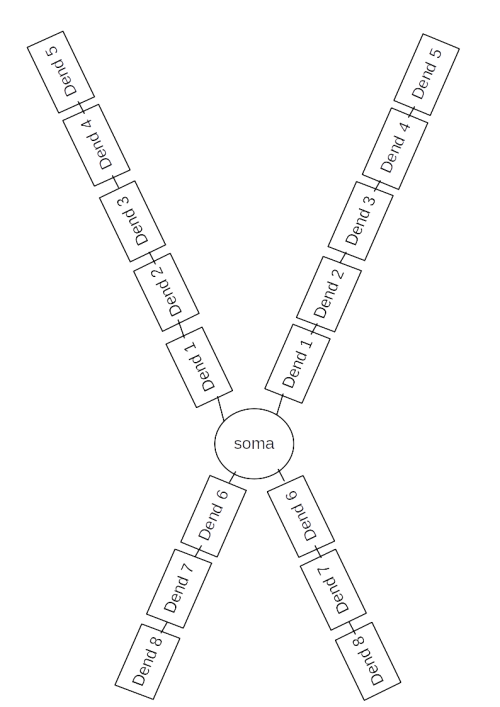
\includegraphics{interneuron_structures.png}
	\caption{Scheme of compartments of sca, ivy, ngf, pvbas, cckbas, aac cells}
	\label{fig:interneuron_structures}
\end{figure}


\begin{figure}[h]
	\centering
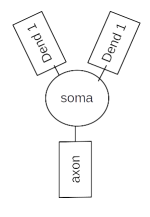
\includegraphics{olm_structure.png}
\caption{Scheme of compartments of olm cell}
\label{fig:olm_structures}
\end{figure}

\begin{figure}[h]
	\centering
	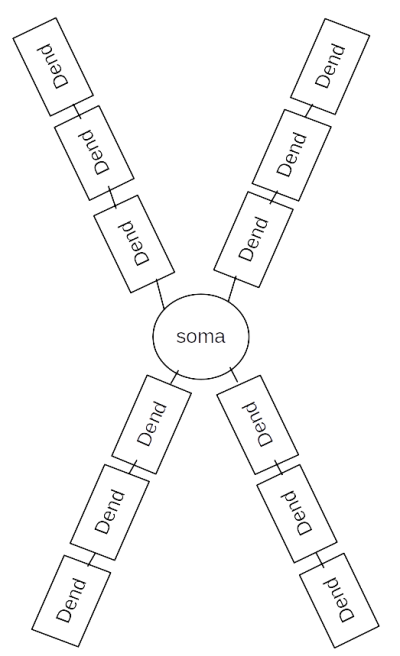
\includegraphics{bis_structure.png}
	\caption{Scheme of compartments of bis cell}
	\label{fig:bis_structures}
\end{figure}


\begin{figure}[h]
	\centering
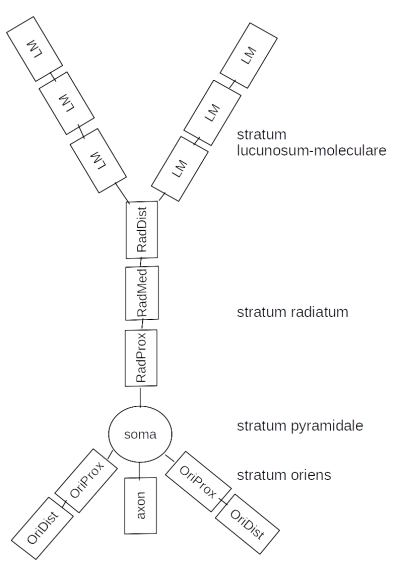
\includegraphics{pyramide_structures.png}
\caption{Scheme of compartments of pyramidal cell}
\label{fig:pyr_structures}
\end{figure}

\section{Synapse models} 
\subsection{General description of synapse models} \label{synapse_models}
We simulate connections  via  gap junctions and chemichal synapses with AMPAR, NMDAR and GABA-A receptors. Model of gap junctions is described in  section (\ref{gap_junctions_models}).
Current trough all synaptic channels is simulated as:
\begin{equation}
I_{syn} = g_{max, syn} \cdot g \cdot (V - E_{syn})
\end{equation}
where $ g_{max, syn}$ is maximal synaptic conduntance in $mS/cm^2$, $g$ is analog of gate variable for synaptic current. $E_{syn}$ is reversal potential in $mV$, for excitatory synapses with AMPA and NMDA receptors $E_{syn} = 0\ mV$, for GABA-A channels $E_{GABA} = -75\ mV$.
Dynamic of $g$ is simulated with double exponetial model: 
\begin{equation}
\label{eq:gsyn}
g = exp \Big( \frac{t - t_0}{\tau_{rise}} \Big) - exp \Big( \frac{t - t_0}{\tau_{decay}} \Big)
\end{equation}
where $t_0$ is time of spike on presynaptic neuron with delay.
NMDAR simulated with equation:
\begin{equation}
I_{NMDA} = g_{max, NMDA} \cdot g \cdot s \cdot (V - E_{NMDA})
\end{equation}
\begin{equation}
s = \frac{1.50265}{1 + 0.33 \cdot exp(-0.0625 \cdot V) }
\end{equation}
where $g$ described by the same equation as AMPAR and GABA-A (\ref{eq:gsyn}).
Parameters $\tau_{rise},\ \tau_{decay}$ for synapses between each group of neurons are described in following sections. For each individual sinapses $g_{max, syn}$ and delay are chosen from lognormal distribution, mean and std are given below.  

\subsection{Synapses from pyramidal cells}
\begin{longtable}{lllllllll}
\caption{Synaptic connections to aac}\label{aac_synapses}\\
\toprule
{} &  $g_{max, mean}$ & $g_{max, \sigma}$ & $\tau_{rise}$ & $\tau_{decay}$ &   $p$ & $delay_{mean}$ & $delay_{\sigma}$ & Compartment \\
\midrule
\endhead
\midrule
\multicolumn{9}{r}{{Continued on next page}} \\
\midrule
\endfoot

\bottomrule
\endlastfoot
bis             &   1.5 &      0.7 &      0.5 &         4 &    0.2 &   1.2 &       0.2 &      dendrite\ \\
ca3\_non\_spatial &   0.7 &      0.2 &        2 &       6.3 &   0.03 &   2.5 &       0.5 &      dendrite\ \\
ca3\_spatial     &   0.7 &      0.2 &        2 &       6.3 &   0.03 &   2.5 &       0.5 &      dendrite\ \\
cckbas          &   0.5 &      0.7 &      0.5 &         4 &    0.2 &   1.2 &       0.2 &      dendrite\ \\
ivy             &   0.5 &      0.7 &      0.5 &         4 &    0.2 &   1.2 &       0.2 &      dendrite\ \\
mec             &     1 &     0.05 &        2 &       6.3 &   0.01 &    10 &       0.5 &      dendrite\ \\
msteevracells   &   0.9 &      0.7 &      0.5 &         3 &    0.5 &  10.5 &       0.5 &               soma \\
olm             &   1.5 &      0.7 &      0.5 &         4 &    0.2 &   1.2 &       0.2 &      dendrite\ \\
pvbas           &   1.5 &      0.7 &      0.5 &         4 &    0.2 &   1.2 &       0.2 &      dendrite\ \\
pyr             &  0.04 &     0.02 &      0.3 &       0.6 &   0.07 &   1.2 &       0.2 &      dendrite\ \\
sca             &   1.5 &      0.7 &      0.5 &         4 &    0.1 &   1.2 &       0.2 &      dendrite\ \\
lec             &   0.1 &     0.05 &        2 &       6.3 &  0.003 &     8 &       0.5 &      dendrite\ \\
\end{longtable}

\begin{longtable}{lllllllll}
\caption{Synaptic connections to bis}\label{bis_synapses}\\
\toprule
{} &   $g_{max, mean}$ & $g_{max, \sigma}$ & $\tau_{rise}$ & $\tau_{decay}$ &  $p$ & $delay_{mean}$ & $delay_{\sigma}$ & Compartment \\
\midrule
\endhead
\midrule
\multicolumn{9}{r}{{Continued on next page}} \\
\midrule
\endfoot

\bottomrule
\endlastfoot
bis    &    0.5 &      0.2 &      0.5 &         4 &   0.5 &   1.2 &       0.2 &      dendrite\ \\
cckbas &    0.5 &      0.2 &      0.5 &         4 &   0.2 &   1.2 &       0.2 &      dendrite\ \\
pvbas  &  0.035 &    0.015 &     0.29 &      2.67 &   0.2 &   1.2 &       0.2 &      dendrite\ \\
pyr    &   0.14 &     0.07 &      1.3 &         8 &  0.14 &   1.2 &       0.2 &      dendrite\ \\
sca    &    0.5 &      0.2 &      0.5 &         4 &  0.05 &   1.2 &       0.2 &      dendrite\ \\
\end{longtable}

\begin{longtable}{lllllllll}
\caption{Synaptic connections to cckbas}\label{cckbas_synapses}\\
\toprule
{} & $g_{max, mean}$ & $g_{max, \sigma}$ & $\tau_{rise}$ & $\tau_{decay}$ &  $p$ & $delay_{mean}$ & $delay_{\sigma}$ & Compartment \\
\midrule
\endhead
\midrule
\multicolumn{9}{r}{{Continued on next page}} \\
\midrule
\endfoot

\bottomrule
\endlastfoot
bis           &    1 &      0.7 &      0.5 &         4 &   0.2 &   1.2 &       0.2 &      dendrite\ \\
cckbas        &  0.2 &      0.2 &      0.2 &       4.2 &  0.63 &   2.7 &       0.5 &      dendrite\ \\
ivy           &  0.5 &      0.2 &      0.5 &         4 &     0 &   1.2 &       0.2 &      dendrite\ \\
msteevracells &  3.5 &      0.2 &      0.5 &         5 &   0.5 &  10.5 &       2.5 &      dendrite\ \\
ngf           &  0.5 &      0.2 &      0.5 &        10 &   0.1 &   1.2 &       0.2 &      dendrite\ \\
olm           &  0.5 &      0.7 &      0.5 &         4 &     0 &   1.2 &       0.2 &      dendrite\ \\
pvbas         &    1 &      0.2 &     0.29 &      2.67 &  0.05 &   1.2 &       0.2 &      dendrite\ \\
\end{longtable}

\begin{longtable}{lllllllll}
\caption{Synaptic connections to ivy}\label{ivy_synapses}\\
\toprule
{} &   $g_{max, mean}$ & $g_{max, \sigma}$ & $\tau_{rise}$ & $\tau_{decay}$ &  $p$ & $delay_{mean}$ & $delay_{\sigma}$ & Compartment \\
\midrule
\endhead
\midrule
\multicolumn{9}{r}{{Continued on next page}} \\
\midrule
\endfoot

\bottomrule
\endlastfoot
cckbas &    0.5 &     0.07 &      0.5 &         4 &   0.1 &   1.2 &       0.2 &      dendrite\ \\
ivy    &    0.5 &      0.2 &      0.5 &         4 &   0.5 &   1.2 &       0.2 &      dendrite\ \\
pvbas  &    0.5 &      0.2 &      0.5 &         4 &   0.5 &   1.2 &       0.2 &      dendrite\ \\
pyr    &  0.041 &    0.021 &      0.3 &       0.6 &  0.13 &   1.2 &       0.2 &      dendrite\ \\
sca    &    3.5 &      0.7 &      0.5 &         4 &   0.2 &   1.2 &       0.2 &      dendrite\ \\
\end{longtable}

\begin{longtable}{lllllllll}
\caption{Synaptic connections to ngf}\label{ngf_synapses}\\
\toprule
{} &  $g_{max, mean}$ & $g_{max, \sigma}$ & $\tau_{rise}$ & $\tau_{decay}$ &  $p$ & $delay_{mean}$ & $delay_{\sigma}$ & Compartment \\
\midrule
\endhead
\midrule
\multicolumn{9}{r}{{Continued on next page}} \\
\midrule
\endfoot

\bottomrule
\endlastfoot
ca3\_non\_spatial &  1.42 &      0.6 &      0.5 &         3 &   0.2 &   1.5 &       0.5 &      dendrite\ \\
ca3\_spatial     &  1.42 &      0.6 &      0.5 &         3 &   0.2 &   1.5 &       0.5 &      dendrite\ \\
ivy             &   0.9 &      0.7 &      3.1 &        42 &   0.8 &   1.2 &       0.2 &      dendrite\ \\
mec             &   1.7 &      0.3 &      0.5 &         3 &   0.3 &  10.2 &       0.2 &      dendrite\ \\
ngf             &  0.75 &      0.7 &      3.1 &        42 &   0.7 &   1.2 &       0.2 &      dendrite\ \\
olm             &  1.27 &      0.6 &      1.3 &      10.2 &   0.4 &   1.2 &       0.2 &      dendrite\ \\
lec             &   0.7 &      0.3 &      0.5 &         3 &  0.05 &   1.2 &       0.2 &      dendrite\ \\
\end{longtable}

\begin{longtable}{lllllllll}
\caption{Synaptic connections to olm}\label{olm_synapses}\\
\toprule
{} &   $g_{max, mean}$ & $g_{max, \sigma}$ & $\tau_{rise}$ & $\tau_{decay}$ &   $p$ & $delay_{mean}$ & $delay_{\sigma}$ & Compartment \\
\midrule
\endhead
\midrule
\multicolumn{9}{r}{{Continued on next page}} \\
\midrule
\endfoot

\bottomrule
\endlastfoot
ivy   &    1.5 &      0.7 &      0.5 &         4 &    0.5 &   1.2 &       0.2 &      dendrite\ \\
msach &    0.5 &      0.1 &      0.5 &         3 &   0.05 &  10.5 &       0.5 &               soma \\
pyr   &  0.031 &   0.0015 &      0.3 &       0.6 &  0.081 &   1.2 &       0.2 &      dendrite\ \\
sca   &    1.5 &      0.7 &      0.5 &         4 &    0.2 &   1.2 &       0.2 &      dendrite\ \\
\end{longtable}

\begin{longtable}{lllllllll}
\caption{Synaptic connections to pvbas}\label{pvbas_synapses}\\
\toprule
{} &  $g_{max, mean}$ & $g_{max, \sigma}$ & $\tau_{rise}$ & $\tau_{decay}$ &  $p$ & $delay_{mean}$ & $delay_{\sigma}$ & Compartment \\
\midrule
\endhead
\midrule
\multicolumn{9}{r}{{Continued on next page}} \\
\midrule
\endfoot

\bottomrule
\endlastfoot
bis             &   1.1 &     0.05 &      0.5 &         4 &   0.5 &   1.2 &       0.2 &      dendrite\ \\
ca3\_non\_spatial &   0.9 &      0.1 &        2 &       6.3 &  0.06 &   1.5 &       0.5 &      dendrite\ \\
ca3\_spatial     &   750 &      0.2 &        2 &       6.3 &   0.6 &   1.5 &       0.5 &      dendrite\ \\
cckbas          &    10 &      0.2 &     0.43 &      4.49 &  0.38 &   4.5 &         2 &               soma \\
ivy             &  10.1 &      0.5 &      0.5 &         4 &   0.8 &   1.2 &       0.2 &      dendrite\ \\
ngf             &     1 &     0.05 &      0.5 &         4 &   0.8 &   1.2 &       0.2 &      dendrite\ \\
olm             &  0.73 &     0.35 &     0.25 &       7.5 &   0.5 &   1.2 &       0.2 &      dendrite\ \\
pvbas           &    10 &     0.01 &      0.8 &       4.8 &   0.7 &   1.2 &       0.2 &               soma \\
pyr             &   0.5 &     0.04 &     0.07 &       0.2 &  0.13 &   1.2 &       0.2 &      dendrite\ \\
sca             &   1.1 &     0.05 &      0.5 &         4 &   0.5 &   1.2 &       0.2 &      dendrite\ \\
\end{longtable}

\begin{longtable}{lllllllll}
\caption{Synaptic connections to pyr}\label{pyr_synapses}\\
\toprule
{} &   $g_{max, mean}$ & $g_{max, \sigma}$ & $\tau_{rise}$ & $\tau_{decay}$ &   $p$ & $delay_{mean}$ & $delay_{\sigma}$ & Compartment \\
\midrule
\endhead
\midrule
\multicolumn{9}{r}{{Continued on next page}} \\
\midrule
\endfoot

\bottomrule
\endlastfoot
aac             &   20.5 &       10 &     0.28 &       8.4 &   0.29 &   1.2 &       0.2 &          axon\ \\
bis             &  0.009 &    0.005 &     0.11 &       9.7 &   0.14 &   1.2 &       0.2 &      dendrite\ \\
ca3\_non\_spatial &    0.1 &    0.002 &      0.5 &         3 &   0.06 &   1.5 &       0.5 &           rad\ \\
ca3\_spatial     &   15.5 &    0.002 &      0.5 &         3 &   0.06 &   1.5 &       0.5 &           rad\ \\
cckbas          &    2.5 &      1.2 &      0.2 &       4.2 &   0.63 &   2.5 &       1.2 &          soma\ \\
ivy             &  0.053 &     0.02 &      1.1 &        11 &   0.13 &   1.2 &       0.2 &            lm\ \\
lec             &   0.06 &    0.007 &      0.5 &         3 &   0.07 &    10 &         2 &            lm\ \\
mec             &   0.06 &    0.007 &      0.5 &         3 &   0.07 &    10 &         2 &            lm\ \\
ngf             &  0.098 &     0.05 &        9 &        39 &   0.29 &   1.2 &       0.2 &            lm\ \\
olm             &    1.7 &      0.9 &     0.13 &        11 &   0.29 &   1.2 &       0.2 &            lm\ \\
pvbas           &     10 &    0.025 &      0.3 &       6.2 &   0.29 &   1.2 &       0.2 &          soma\ \\
pyr             &      5 &    0.007 &      0.1 &       1.5 &  0.009 &   1.2 &       0.2 &         basal\ \\
sca             &  0.098 &     0.05 &      0.3 &       6.2 &   0.29 &   1.2 &       0.2 &           rad\ \\
\end{longtable}

\begin{longtable}{lllllllll}
\caption{Synaptic connections to sca}\label{sca_synapses}\\
\toprule
{} &  $g_{max, mean}$ & $g_{max, \sigma}$ & $\tau_{rise}$ & $\tau_{decay}$ &  $p$ & $delay_{mean}$ & $delay_{\sigma}$ & Compartment \\
\midrule
\endhead
\midrule
\multicolumn{9}{r}{{Continued on next page}} \\
\midrule
\endfoot

\bottomrule
\endlastfoot
bis             &   0.5 &      0.2 &      0.5 &         4 &   0.1 &   1.2 &       0.2 &      dendrite\ \\
ca3\_non\_spatial &  0.05 &     0.02 &      0.5 &         4 &  0.09 &   1.2 &       0.2 &      dendrite\ \\
ca3\_spatial     &  0.05 &     0.02 &      0.5 &         4 &  0.09 &   1.2 &       0.2 &      dendrite\ \\
ivy             &   0.5 &      0.2 &      0.5 &         4 &   0.1 &   1.2 &       0.2 &      dendrite\ \\
ngf             &   0.5 &      0.2 &      0.5 &         4 &   0.2 &   1.2 &       0.2 &      dendrite\ \\
olm             &   1.3 &      0.6 &     0.07 &        29 &   0.1 &   1.2 &       0.2 &      dendrite\ \\
sca             &  0.03 &    0.015 &        4 &      34.3 &   0.3 &   1.2 &       0.2 &      dendrite\ \\
\end{longtable}


\begin{longtable}{lllllll}
\caption{Parameters of NMDAR in the exite synapses}\label{nmda_parameters}\\
\toprule
 Presynaptic & Postsynaptic & $g_{max, mean}, \ mS$ & $g_{max, \sigma}$ & $\tau_{rise}, \ ms$ & $\tau_{decay}, \ ms$ & $E_{NMDA}$, \ mV \\
\midrule
\endhead
\midrule
\multicolumn{7}{r}{{Continued on next page}} \\
\midrule
\endfoot

\bottomrule
\endlastfoot
 ca3\ &        pvbas &     0.03 &    0.001 &  2.3 &    95 &     0 \\
 ca3\ &          pyr &     0.05 &    0.001 &  2.3 &    95 &     0 \\
         pyr &        pvbas &     0.01 &    0.001 &  2.3 &    95 &     0 \\
         pyr &          pyr &     0.05 &    0.001 &  2.3 &    95 &     0 \\
\end{longtable}


\section{Gap junction models} \label{gap_junctions_models}
\subsection{General description of gap junction models}
Gap junction between two neurons (1 and 2) is described by simple equation:
\begin{equation}
I_{gap} = \frac{V_{1} - V_{2}}{R_{gap}}
\end{equation}
where $I_{gap}$ is current for neuron 1, $V_{1}$ and $V_{2}$ are potentials of neuron 1 and 2 respectivly. Gap junctions are always simmetrical, in equation of neuron 2 same current is added. $R_{gap}$ is resistance of contact, it is chosen randomly from normal disrtibuntion for each contact, parameters see below.


\begin{longtable}{lllrl}
\caption{Parameters of gap junctions}\label{gap_junctions_parameters}\\
\toprule
Celltype &   $R_{gap, mean}$ &  $R_{gap, \sigma}$ &  $p$ &   Compartment \\
\midrule
\endhead
\midrule
\multicolumn{5}{r}{{Continued on next page}} \\
\midrule
\endfoot

\bottomrule
\endlastfoot
     ngf &  100000 &  10000 &   0.7 &  dendrite\ \\
   pvbas &  100000 &  10000 &   0.1 &  dendrite\ \\
\end{longtable}




\section{Simulation of local field potetial} \label{field_potetial_model}
LFP simulated with LFPsim tools, we have used line aproximation:
\begin{equation} 
\Phi_{LFP} = \sum^{n}_{i=1}{ \frac{I_i}{2\pi \sigma}log \Big(\frac{\sqrt{h_i^2 + r_i^2}-h_i}{\sqrt{l_i^2 + r_i^2}-l_i} } \Big)
\end{equation}
$\Phi_{LFP}$ is simulated LFP, $I$ is transmemrane current.
In simulation of LFP only comratmments of pyramidal neurons were taken into account. $\sigma$ denotes
the conductivity of the medium. $r$ is the distance from
source to the point of measurement, $h$ is the distance from end of segment to point of measurement, $l$ is the length of secgment. All the pyramid neurons were arranged in an orderly fashion. The soma of all the cells were on the same level ($z=0$). The $x$ and $y$ coordinates for each neuron were chosen randomly from the circe with radius $R_{x, y}$ specified by the formula:
\begin{equation} 
R_{x, y} = \frac{\sqrt{\frac{N_{pyr}}{\rho_{pyr}} }} {\pi}
\end{equation}
where $N_{pyr}$ is the number of pyramidal cells in model, $\rho_{pyr} = 0.2 \ cell/\mu m^2$ is the dencity of cells in pyramidal layer of the CA1 field.


%\bibliography{bibliography}
\end{document}



